\documentclass[../uilmath.tex]{subfiles}
\graphicspath{{\subfix{../figures/}}}
\begin{document}
\chapter{Extra Topics}
\section*{Problems}
\begin{enumerate}[label=\bfseries\arabic*.]
    \item %% Problem 1
    Which equality axiom of addition is demonstrated by $(ax+by)+c=ax+(by+c)$?

    \item %% Problem 2
    Which of the following numbers is considered to be an ``abundant'' number?

    $\textbf{(A) } 26 \qquad \textbf{(B) } 28 \qquad \textbf{(C) } 30 \qquad \textbf{(D) } 32 \qquad \textbf{(E) } 34$

    \item %% Problem 3
    $ABC1_{16}+ABC1_{15}=\blank_{14}$

    \item %% Problem 4
    Let $P={2,3,5}, Q={2,4,6}$, and $R={3,5,7}$. How many elements are in $(P\cap R)\cup(R\cap Q)$?

    \item %% Problem 5
    Which of the following sets is closed under addition and subtraction?

    $\textbf{(A) } \text{Positive Even Numbers} \qquad \textbf{(B) } \text{Integers} \qquad \textbf{(C) } \text{Positive Odd Numbers} \qquad \textbf{(D) } \text{Primes} \qquad \textbf{(E) } \text{Wholes}$

    \item %% Problem 6
    Find the harmonic mean of 4 and 9.

    \item %% Problem 7
    Which of the following numbers is considered to be an ``deficient'' number?

    $\textbf{(A) } 24 \qquad \textbf{(B) } 56 \qquad \textbf{(C) } 66 \qquad \textbf{(D) } 92 \qquad \textbf{(E) } 112$

    \item %% Problem 8
    In the decimal number $2x3y4z$, the letters $x$, $y$, and $z$ represent digits where all six digits are distinct.
    If the number is divisible by 30 then $x+y+z$ could be: 

    \item %% Problem 9
    $888_9 + 555_6 + 222_3 = \blank_3$

    \item %% Problem 10
    Use the Fibonacci characteristic sequence $\dots -1.5,p,q,3,r,\dots$ to Find $p+q+r$.

    \item %% Problem 11
    One of Eratosthenes of Cyrene's main contributions to mathematics involved a method for finding \blank .

    \item %% Problem 12
    I'm an unhappy deficient number but a number that is lucky to be prime. Which of the following numbers am I?

    \item %% Problem 13
    Which equality axiom of multiplication is demonstrated by $(a)(a)^{-1}=1$?

    \item %% Problem 14
    How many subsets containing 4 members can be made from the set ${2,1,3,4,7,11}$?

    \item %% Problem 15
    Which of the following was the first Nigerian woman to be awarded a doctorate in mathematics?

    \item %% Problem 16
    Find the harmonic mean of the roots of $x^3-7x^2+14x-8=0$.

    \item %% Problem 17
    If $R$, $S$, and $T$ are distinct digits then $RST_2-ST_3-R_4$ has a numeric value in base 10 of:

    \item %% Problem 18
    The set ${\dots, -6, -4,-2,0,2,4,6,\dots}$ is closed under which of the following operations:
    \begin{center}
        I. addition \qquad II. subtraction \qquad III. multiplication \qquad IV. division 
    \end{center}

    \item %% Problem 19
    $F_0=0$ and $F_1$ are the first two Fibonacci numbers. Find $F_{10}$.

    \item %% Problem 20
    Let $R={1,3,5}, S={0,2,4}$, and $T={1,2,3}$. How many elements are in $(R\cup T)\cap(S\cup T)$?

    \item %% Problem 21
    $(p-q)\times r = pr-qr$ is an example of which property of equality?

    \item %% Problem 22
    The 8th Fibonacci number is 13. The 10th Fibonacci number is 34. Find the 9th Lucas number.

    \item %% Problem 23
    Find $L_9$ if $L_0=2,L_1=1$, and $L_n=L_(n-1)+L_(n-2)$, where $n\geq 2$.

    \item %% Problem 24
    The universal set $U={2,3,5,7,11,13,15,17,19}$. Subset $L={5,7,15,17}$, subset $M={3,13}$. 
    How many elements are in the complement set of $L\cup M$?

    \item %% Problem 25
    Which of the following mathematicians was most remembered as the inventor of logarithms?

    \item %% Problem 26
    In the binomial expansion of $(3x-1)^5$, the coefficient of the fourth term is:

    \item %% Problem 27
    What are the odds that a factor of 2010 is a prime number?

    \item %% Problem 28
    The formula $e^{ix}=\cos x + i\sin x$, where $e$ is the base of the natural logarithm and $i$ is the imaginary unit, is named after:

    \item %% Problem 29
    The odd numbers from 1 to 17 are to be placed in this magic square in which the rows and columns have the same sum. Find the value of $x$.
    \begin{center}
        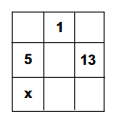
\includegraphics[width=0.3\textwidth]{2010A28.PNG}
    \end{center}

    \item %% Problem 30
    $P={p,l,u,s}, Q={m,i,n,u,s}$, and $R={t,i,m,e,s}$. How many elements are in $(P\cup Q)\cap (P\cup R)$?

    \item %% Problem 31
    The number 12010 in base 3 is equivalent to the number $wxyz$ in base 5, where $w$, $x$, $y$, and $z$ are digits. Find $w+x+y+z$.

    \item %% Problem 32
    $3(x+4)=5$ and $3(4+x)=5$ is an example of the \blank property.

    \item %% Problem 33
    If $ax+b=c$ and $c=dx+e$, then $ax+b=dx+e$ is an example of the \blank property.

    \item %% Problem 34
    Which of the following is true about the relation graphed below?
    \begin{center}
        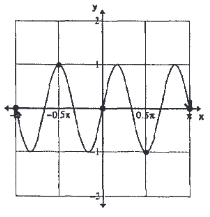
\includegraphics[width=0.3\textwidth]{2010B16.PNG}
    \end{center}

    \item %% Problem 35
    Integers $x$ \& $y$ exist such that $x=2y$ and the arithmetic mean of $x$ \& $y$ is 1 more than the harmonic mean of $x$ \& $y$. Find the geometric mean of $x$ \& $y$.

    \item %% Problem 36
    The figure shown is reflected over a negative diagonal. Which of the following figures is the result of that single transformation?
    \begin{center}
        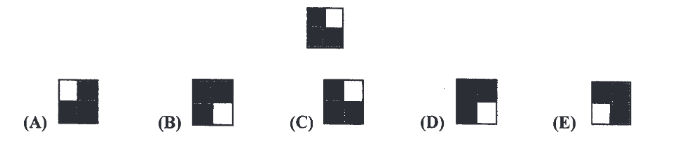
\includegraphics[width=0.7\textwidth]{2010B23.PNG}
    \end{center}

    \item %% Problem 37
    A recent visit to the planet Strangebase discovered that the equation, $3S^2-25S+66=0$, has two solutions, 4 and 9. What base was being used for the number system on planet Strangebase?

    \item %% Problem 38
    Evaluate: $\prod_{n=2}^6 (1+\frac{1}{n})$

    \item %% Problem 39
    Which of the following mathematicians created an abacus for calculating products and quotients and extracting square roots that was based on Arab mathematics and lattice multiplication.

    \item %% Problem 40
    Polly Euler folds the net shown into a cube. What letter will be on the opposite side of side $S$?
    \begin{center}
        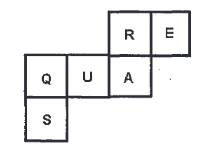
\includegraphics[width=0.3\textwidth]{2010B34.PNG}
    \end{center}

    \item %% Problem 41
    If $\sqrt{x\sqrt[3]{x\sqrt[4]{x}}}=\sqrt[n]{x^k}$, where $k$ and $n$ are relatively prime, then $k=$?

    \item %% Problem 42
    The universal set $U={1,2,3,5,8,13,21,34}$. Subset $A={1,3,8,21,34}$ and subset $B={2,3,5,13,21}$. How many elements are in the complement set of $A\cap B$?

    \item %% Problem 43
    Which of the following numbers is an unhappy number and evil number?

    $\textbf{(A) } 7 \qquad \textbf{(B) } 8 \qquad \textbf{(C) } 9 \qquad \textbf{(D) } 10 \qquad \textbf{(E) } 11$

    \item %% Problem 44
    
\end{enumerate}

\section*{Solutions}
\begin{enumerate}[label=\bfseries\arabic*.]
    \item %% Problem 1
    Associative 

    \item %% Problem 2
    C  

    \item %% Problem 3
    21411

    \item %% Problem 4
    2

    \item %% Problem 5
    B 

    \item %% Problem 6
    $5 \frac{7}{13}$

    \item %% Problem 7
    D 

    \item %% Problem 8
    12 

    \item %% Problem 9
    689

    \item %% Problem 10
    6.75

    \item %% Problem 11
    prime numbers 

    \item %% Problem 12
    37

    \item %% Problem 13
    Commutative

    \item %% Problem 14
    15

    \item %% Problem 15
    Grace Alele Williams 

    \item %% Problem 16
    $1\frac{5}{7}$

    \item %% Problem 17
    $3R-S$

    \item %% Problem 18
    I, II \& III 

    \item %% Problem 19
    55

    \item %% Problem 20
    3

    \item %% Problem 21
    distributive 

    \item %% Problem 22
    47

    \item %% Problem 23
    76

    \item %% Problem 24
    3

    \item %% Problem 25
    John Napier 

    \item %% Problem 26
    -90

    \item %% Problem 27
    $\frac{1}{3}$

    \item %% Problem 28
    Leonard Euler 

    \item %% Problem 29
    7

    \item %% Problem 30
    6

    \item %% Problem 31
    6

    \item %% Problem 32
    commutative 

    \item %% Problem 33
    distributive

    \item %% Problem 34
    It is a one-to-one function.

    \item %% Problem 35
    $3\sqrt{2}$

    \item %% Problem 36
    D 

    \item %% Problem 37
    base 5 

    \item %% Problem 38
    11.39 

    \item %% Problem 39
    Sophie Germain 

    \item %% Problem 40
    A 

    \item %% Problem 41
    12 

    \item %% Problem 42
    6

    \item %% Problem 43
    C 

    \item %% Problem 44
    
\end{enumerate}

\end{document}